\documentclass[]{article}
\renewcommand{\baselinestretch}{1.25}

\usepackage[margin=1in]{geometry}
\usepackage{physics}
\usepackage{amsmath, amsfonts, amssymb, amsthm}
\usepackage{amssymb}
\usepackage{graphicx}
\usepackage{hyperref}
\usepackage{empheq}
\usepackage{pdfpages}
\usepackage{xcolor}
\usepackage{ulem}

% MATLAB Formatting Code
\usepackage[numbered,framed]{matlab-prettifier}
\lstset{style=Matlab-editor,columns=fullflexible}
\renewcommand{\lstlistingname}{Script}
\newcommand{\scriptname}{\lstlistingname}

% TikZ Things
\usepackage{tikz}
\usetikzlibrary{positioning,shapes}


% Formatting Preferences
\numberwithin{equation}{section}
\usepackage{parskip}
\renewcommand{\figurename}{Fig.}
\allowdisplaybreaks

% Section Heading Settings
\usepackage{enumitem}
\renewcommand{\theenumi}{\alph{enumi}}
\renewcommand*{\thesection}{Problem \arabic{section}}
\renewcommand*{\thesubsection}{\alph{subsection})}
\renewcommand*{\thesubsubsection}{\quad \quad \roman{subsubsection})}

% Math Proof things
\newcommand{\Rel}{\mathcal{R}}
\newcommand{\R}{\mathbb{R}}
\newcommand{\C}{\mathbb{C}}
\newcommand{\N}{\mathbb{N}}
\newcommand{\Z}{\mathbb{Z}}
\newcommand{\Q}{\mathbb{Q}}

\newcommand{\st}{\ : \ }

% Theorem Definition
\newtheorem{definition}{Definition}
\newtheorem{assumption}{Assumption}
\newtheorem{theorem}{Theorem}
\newtheorem{lemma}{Lemma}
\newtheorem{proposition}{Proposition}
\newtheorem{example}{Example}


% Multiagent Robotic Systems Commands
\newcommand{\diam}{\textnormal{diam}}
\newcommand{\radius}{\textnormal{radius}}




%opening
\title{MECH 6V29: Multiagent Robotic Systems- HW 2}
\author{Jonas Wagner}
\date{2022, March 1\textsuperscript{st}}

\begin{document}	

\maketitle

\tableofcontents

%----------------------------------------------------------------------------

% Problem 1 -------------------------------------------------
\newpage
\section{}
% \textbf{Problem:} 
State a summary of lectures \emph{\textbf{lectures 6-10}}, preferably by creating a concept map diagram (flow diagram). 
The whole purpose is to make sure that we are clear about the bigger picture, 
and reiterate why are we doing and discussing the specific topics in the class. 
Do not merely write the topics, instead create connections between topics to clarify the flow of information.

\subsection{Big Picture Chart}
\begin{figure}[h]
	\centering
    \resizebox*{\textwidth}{!}{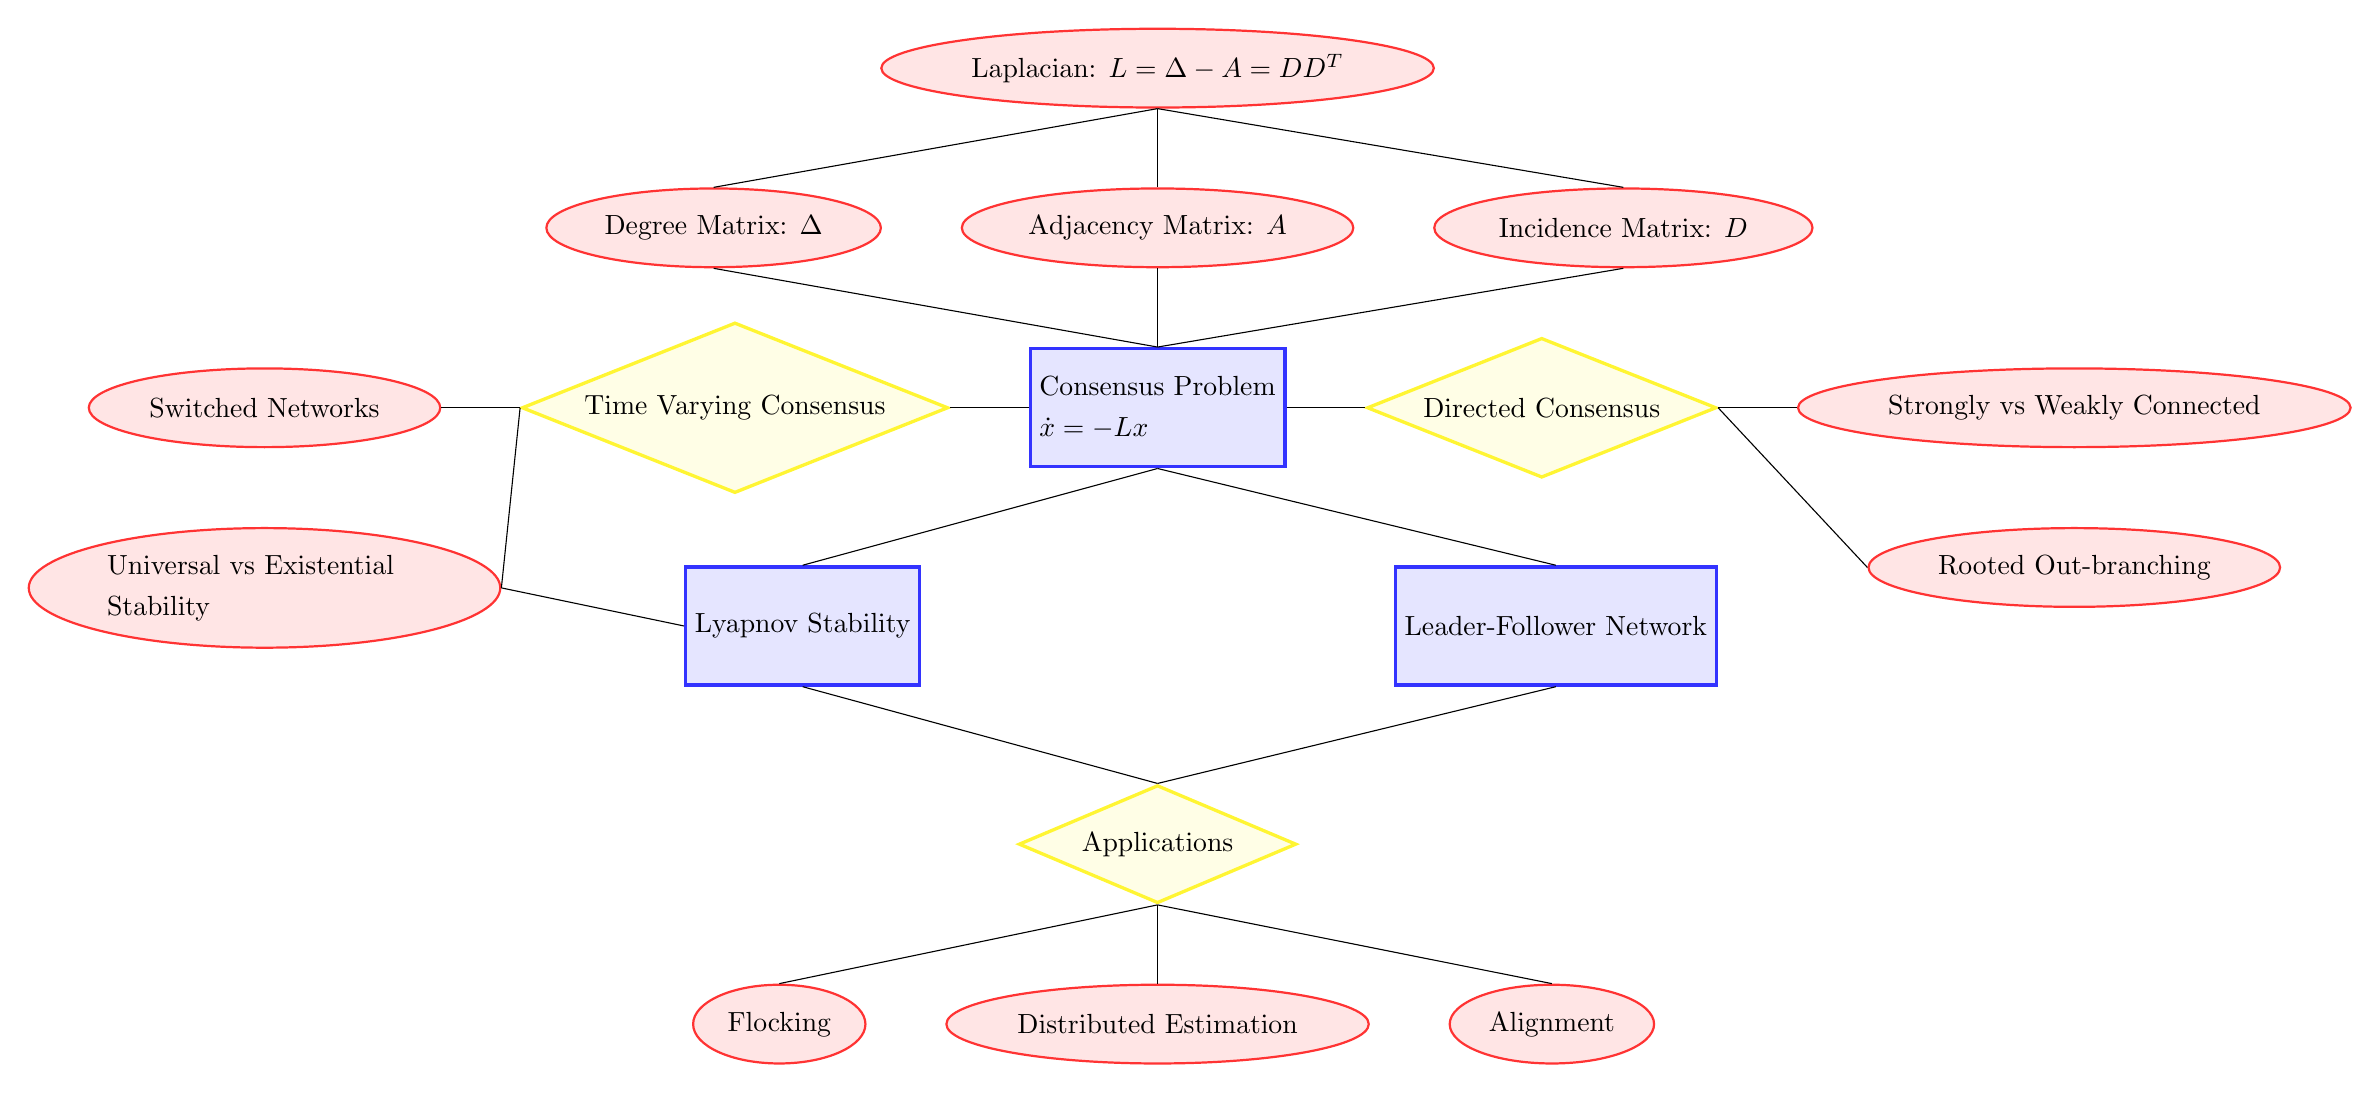
\begin{tikzpicture}[
		empty/.style={coordinate, draw=white!0, fill=white!0, thin, minimum size = 0.1mm},
		block/.style={rectangle, draw=blue!80, fill=blue!10, very thick, minimum size = 15mm},
        subblock/.style={diamond, draw=yellow!80, fill=yellow!10, very thick, minimum size = 15mm, aspect=2.5},
		extra/.style={ellipse, draw=red!80, fill=red!10, thick, minimum size = 10mm},
		auto,
		% roundnode/.style={circle, draw=green!60, fill=green!5, very thick, minimum size=7mm},
		% squarednode/.style={rectangle, draw=red!60, fill=red!5, very thick, minimum size=5mm},
		]
		%Main Nodes
		\node[empty]	(center)								{};
		
        %Consensus
        \node[block, text width = 30mm]	(consensus)	[above=2cm of center]	{Consensus Problem $\dot{x}=-L x$};
        \node[extra]	(con_2)		[above=of consensus]	{Adjacency Matrix: $A$};
        \node[extra]	(con_1)		[left=of con_2]			{Degree Matrix: $\Delta$};
        \node[extra]	(con_3)		[right=of con_2]		{Incidence Matrix: $D$};
        \node[extra]	(con_4)		[above=of con_2]		{Laplacian: $L = \Delta - A = DD^T$};
        \draw[-]	(consensus.north) 	--	(con_1.south);
        \draw[-]	(consensus.north) 	--	(con_2.south);
        \draw[-]	(consensus.north) 	--	(con_3.south);
        \draw[-]	(con_1.north)		--	(con_4.south);
        \draw[-]	(con_2.north)		--	(con_4.south);
        \draw[-]	(con_3.north)		--	(con_4.south);

        %Directed Consensus
        \node[subblock]	(di_con)	[right=of consensus]	{Directed Consensus};
        \draw[-]    (consensus.east) -- (di_con.west);
        \node[extra]    (di_con_1)  [right=of di_con]    {Strongly vs Weakly Connected};
        \draw[-]    (di_con.east) -- (di_con_1.west);
        \node[extra]    (di_con_2)  [below=of di_con_1]    {Rooted Out-branching};
        \draw[-]    (di_con.east) -- (di_con_2.west);

        %Time-Varying Consensus
        \node[subblock]	(tv_con)	[left=of consensus]	{Time Varying Consensus};
        \draw[-]    (consensus.west) -- (tv_con.east);
        \node[extra]    (tv_con_1) [left=of tv_con] {Switched Networks};
        \draw[-]    (tv_con.west) -- (tv_con_1.east);
        \node[extra, text width = 40mm]    (tv_con_2) [below=of tv_con_1] {Universal vs Existential Stability};
        \draw[-]    (tv_con.west) -- (tv_con_2.east);

        %Lyapnov Stability
        \node[block]	(lyap)		[left=3cm of center] 	{Lyapnov Stability};
        \draw[-]    (lyap.west) -- (tv_con_2.east);
        \draw[-]    (lyap.north) -- (consensus.south);

        %Leader-Follower System
        \node[block]	(lead_follow)		[right=3cm of center] 	{Leader-Follower Network};
        \draw[-] (consensus.south) -- (lead_follow.north);

		%Applications
        \node[subblock] (app) [below=2cm of center] {Applications};
        \draw[-] (lead_follow.south) -- (app.north);
        \draw[-] (lyap.south) -- (app.north);
		\node[extra]	(app_2)		[below=of app]	    {Distributed Estimation};
		\node[extra]	(app_1)		[left=of app_2]		{Flocking};
		\node[extra]	(app_3)		[right=of app_2]	{Alignment};
		\draw[-]	(app.south) -- (app_1.north);
		\draw[-]	(app.south) -- (app_2.north);
		\draw[-]	(app.south) -- (app_3.north);
	\end{tikzpicture}}
	\caption{Diagram of Course Topics (created w/ TikZ)}
	\label{fig:pblm1}
\end{figure}

% Problem 2 -------------------------------------------------
\newpage
\section{}
Recall that if $x_i$ is scalar, with its derivative given by the consensus equation \[
    \dot{x}_i = \sum_{j \in \mathcal{N}_i} (x_j - x_i), \ i = 1, 2, \cdots, N
\] this can be written as \[
    \dot{x} = - L x
\] where $L$ is the Laplacian of the undirected graph, 
and $x = \mqty[x_1 x_2 \cdots x_N]^T$.

\subsection{}
\subsubsection*{Problem:}
If instead\[
    \dot{x} = - L^2 x
\] what are the corresponding node level dynamics, that is, find \[
    \dot{x}_i = ???
\]
\subsubsection*{Preliminaries}
\begin{definition} \label{def:graph_matrices}
	Let graph $G(V,E)$ with $V = \qty{v_1,\dots,v_n}$ and $E \subseteq V \cross V$.
	\begin{enumerate}
		\item The \underline{\emph{degree matrix}} $\Delta \in \R^{n\cross n}$ is a diagonal matrix defined as \[
			\Delta := \mqty[\dmat{\deg(v_1), \deg(v_2), \ddots, \deg(v_n)}]
		\]
		\item The \emph{\underline{adjacency matrix}} $A \in \R^{n\cross n}$ is a symmetric matrix $(A = A^T)$ defined s.t. \[
			A = [a_{ij}] \st a_{ij} \begin{cases}
				1 &(v_i,v_j) \in V\\
				0 &(v_i,v_j) \notin V
			\end{cases}
		\]
		\item The \emph{\underline{incidence matrix}} $D \in \R^{n \cross m}$ is defined as\[
			D = [d_{ij}] \st d_{ij} \begin{cases}
				1 	&(v_i,-) \in e_{j}\\
				-1	&(-,v_i) \in e_{j}\\
				0	&\text{otherwise}
			\end{cases}
		\]
		\item The \emph{\underline{Laplacian matrix}} $L \in \R^{n \cross n}$ is a symmetric $(L = L^T)$ and strictly semi-positive definite $(L \succeq 0)$ is defined as\[
			L := \Delta - A = D D^T
		\]and\[
			L = \mqty[
				\deg(v_1)	&-a_{12}	&-a_{13}	&\cdots	&-a_{1n}\\
				-a_{21}		&\deg(v_2)	&-a_{23}	&\cdots	&-a_{2n}\\
				\vdots		&\vdots		&\vdots		&\ddots	&\vdots\\
				-a_{n1}		&-a_{n2}	&-a_{n3}	&\cdots	&\deg(v_n)
			]
		\]
		\item For a weighted graph $G(V,E,W)$, the diagonal weighted matrix $W\in \R^{m\cross m}$ is defined as\[
			W = [w_{ij}] \forall_{ij \in E}
		\]
		were $w_{ij}$ are the corresponding weights for $e_{ij} = (v_i,v_j)$.
	\end{enumerate}
\end{definition}

\begin{definition} \label{def:consensus_dynamics}
	Let undirected and unweighted graph $G(V,E)$ with $V = \qty{v_1,\dots,v_n}$ and $E \subseteq V \cross V$.
	The \emph{\underline{consensus dynamics}} of network $G(V,E)$ is defined by\[
		\forall_{i=1,\dots,n} \ \dot{x}_i = \sum_{j\in \mathcal{N}_i} (x_j - x_i)
		\iff \dot{x} = -L x
	\] For the case with weighted graph $G(V,E,W)$ with diagonal weight matrix $W = [w_{ij}]$, 
	\emph{\underline{weighted consensus dynamics}} are given as\[
		\dot{x}_i = \sum_{j\in\mathcal{N}_i} w_{ij} (x_j - x_i) 
		\implies \dot{x} = - L_{w} x
	\]where weighted Laplacian matrix $L_{w}$ is defined as\[
		L_{w} = D W D^T
	\]
\end{definition}

\subsubsection*{Solution:}
From the definition of the Laplacian Matrix (Definition \ref{def:graph_matrices}), we have\[
    L = \Delta - A
\] and therefore \begin{align*}
    L^2 &= L * L = (\Delta - A) (\Delta - A)\\
        &= \Delta^2 - \Delta A - A \Delta + A^2\\
        &= \mqty[
            \deg(v_1)^2	&0	&0	&\cdots	&0\\
            0		&\deg(v_2)^2	&0	&\cdots	&0\\
            \vdots		&\vdots		&\vdots		&\ddots	&\vdots\\
            0		&0	&0	&\cdots	&\deg(v_n)^2
        ] \\ &\qquad + \mqty[
            0	&-a_{12} \deg(v_1)	&-a_{13} \deg(v_1)	&\cdots	&-a_{1n} \deg(v_1)\\
            -a_{21}	\deg(v_2)	&0	&-a_{23} \deg(v_2)	&\cdots	&-a_{2n} \deg(v_2)\\
            \vdots		&\vdots		&\vdots		&\ddots	&\vdots\\
            -a_{n1}	\deg(v_n)	&-a_{n2} \deg(v_n)	&-a_{n3} \deg(v_n)	&\cdots	&0
        ] \\ &\qquad + \mqty[
            0	&-a_{12} \deg(v_1)	&-a_{13} \deg(v_2)	&\cdots	&-a_{1n} \deg(v_3)\\
            -a_{21}	\deg(v_1)	&0	&-a_{23} \deg(v_2)	&\cdots	&-a_{2n} \deg(v_3)\\
            \vdots		&\vdots		&\vdots		&\ddots	&\vdots\\
            -a_{n1}	\deg(v_1)	&-a_{n2} \deg(v_2)	&-a_{n3} \deg(v_3)	&\cdots	&0
        ] \\ &\qquad + \mqty[
            \sum_{i \neq 1}^n a_{1,i} a_{i,1} & \sum_{i \neq 1,2} a_{1,i} a_{i,2} & \cdots &\sum_{i \neq 1,n} a_{1,i} a_{i,2}\\
            \sum_{i \neq 2,1} a_{2,i} a_{i,1} & \sum_{i \neq 2} a_{2,i} a_{i,2} & \cdots & \sum_{i \neq 1,n} a_{1,i} a_{i,n}\\
            \vdots  &  \vdots &\ddots &\vdots\\
            \sum_{i \neq n,1} a_{n,i} a_{i,1} & \sum_{i \neq n,2} a_{n,i} a_{i,2} &\cdots &\sum_{i\neq n} a_{n,i} a_{i,n}
        ]
\end{align*}
which results in \[\boxed{
    \dot{x}^{(i)} = - \qty(\deg(v_1)^2 + \sum_{j \neq i} a_{i,j} a_{j,i}) x^{(i)} 
                    - \sum_{j \neq i} \qty(-a_{i,j} (\deg(v_i) + \deg(v_j)) + \sum_{k \neq j} a_{i,k} a_{k,j}) x^{(j)}
}\]


\subsubsection*{\textcolor{red}{Updated Solution:}}
\[
    p = L x \iff p_i = \sum_{j \in \mathcal{N}_i} (x_i - x_j)
\]\[
    q = L p \iff q_i = \sum_{j \in \mathcal{N}_i} px_i - p_j)
\]\[
    \dot{x} = - L^2 x = - q 
        \iff \dot{x}_i = - \sum_{j \in \mathcal{N}_i} \qty(
            \sum_{k \in \mathcal{N}_i} (x_i - x_k)
            - \sum_{l \in \mathcal{N}_j} (x_j - x_l)
        )
\]

\subsection{}
\subsubsection*{Problem:}
Can you give a graph-theoretic interpretation to your answer in $(A)$?


\subsubsection*{Solution:}
A potential graph-theoretical interpretation could be would be a network with nonlinear consensus dynamics dependent on more then just a single dynamic link. 
This is particularly interesting when looking at representations of digital logic gates or neuron type "circuitry".

\subsubsection*{\textcolor{red}{Updated Solution:}}
The 'nonlinear consensus dynamics' I refereed to are essentially just that the difference between the neighbors of neighbors are included in consensus as well.


% Problem 3 -------------------------------------------------
\newpage
\section{}
Consider a leader-follower network with two leaders and two followers, as shown in \figurename \ref{fig:pblm3}. 
Assume that leaders and followers are on the real line, and the underlying network graph is a path graph with the end nodes being the static leaders.
Moreover, let the dynamics be given by the following:
\begin{gather*}
    \dot{x}_1 = \alpha_1((x_3-x_1) + (x_2 - x_1))\\
    \dot{x}_2 = \alpha_2((x_1-x_2) + (x_4 - x_2))\\
    \dot{x}_3 = \dot{x}_4 = 0
\end{gather*}
Where to $x_1$ and $x_2$ end up as $t \to \infty$ if $x_3 = \beta$ and $x_4 = \gamma$?

\begin{figure}[h]
    \centering
    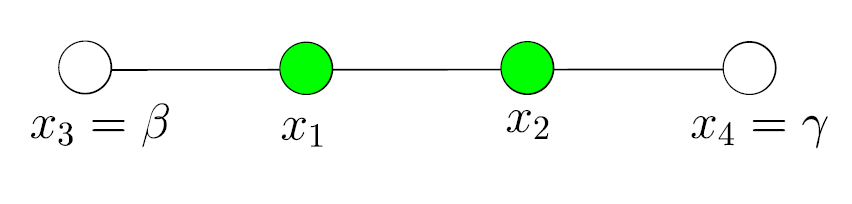
\includegraphics[width=0.7\textwidth]{figs/pblm3.png}
    \caption{Leader-follower Network}
    \label{fig:pblm3}
\end{figure}

\subsection*{Solution:}
The dynamics of the network overall are described by the dynamics $\dot{x} = A_cls x$ with matrix \[
    A_{cls} = \mqty[
        -2 \alpha_1 & \alpha_1 & \alpha_1 &0\\
        \alpha_2 & - 2 \alpha_2 & 0 & \alpha_2\\
        0  & 0 & 0 & 0\\
        0  & 0 & 0 & 0
    ]
\] This can further be redefined into the dynamical system $\dot{x} = A x + B u$ with matrices \[
    A = \mqty[
        -2 \alpha_1 & \alpha_1\\
        \alpha_2    & -2 \alpha_2
    ]
\] \[
    B = \mqty[\dmat{
        \alpha_1,
        \alpha_2
    }]
\] where $u$ is the static "input" of \[
    u = \mqty[
        \beta\\
        \gamma
    ]
\]

Assuming that $\alpha_1, \alpha_2 > 0$, $A$ is stable and therefore the system wll decay to the reference signal $u$.
\emph{Note:} If $u$ changes then the response would be governed by transfer function $(s I - A)^{-1} B$.
The final state will be the solution to \[
    \dot{x} = 0 = A_{cls} x = A x + B u
\] which is calculated to be \[\boxed{
    x_{\infty} = \mqty[
        \cfrac{2 \beta + \gamma}{3}\\
        \cfrac{\beta + 2 \gamma}{3}
    ]
}\]
    

% Problem 4 -------------------------------------------------
\newpage
\section{}
\subsection*{Problem:}
Given an undirected network containing a total of $N$ nodes. 
There is a single anchor node that is connected to every one of the follower nodes, that is, anchor has a degree of $N-1$. 
Find the simple expression for the following quantities.
\begin{enumerate}
    \item $l$
    \item $L_f \vb{1}$
\end{enumerate}
where $L_f$ is the matrix obtained from the partition of the Laplacian matrix as we discussed in class.

Also, relate your answers to where the followers end up as $t \to \infty$.

\subsection*{Preliminaries:}
\begin{definition}\label{def:leader_follower_dynamics}
    Let undirected and unweighted graph $G(V,E)$ with $V = \qty{v_1,\dots,v_n}$ and $E \subseteq V \cross V$.
    Vertices in $V$ are classified as either \emph{leaders} ($v_i \in V_l$) or \emph{followers} ($v_i \in V_f)$. 
	The \emph{\underline{leader-follower}} dynamics of the states within network $G(V,E)$ are defined by\[\begin{cases}
        \dot{x}_i = - \sum_{j \neq N_i} (x_i - x_j) &\forall_{i \st v_i \in V_{f}}\\
        \dot{x}_i =  0 &\forall_{i \st v_i \in V_{l}}
    \end{cases}
	\] or equivalently when $V_{l} = \{v_n\}$ (single leader node) \[
        \dot{x} = \mqty[
            -L_f & - l\\
            0 & 0
        ]
    \]
\end{definition}

\subsection*{Solution:}
Assuming that the network is unweighted and the single leader is associated with $v_n$,\[
    \dot{x} = \mqty[
        -L_f & - l\\
        0 & 0
    ]
\]
\subsubsection{$l$}
Since $\deg(v_n) = N-1$, \[
    \sum_{i=1}^{N-1} l_i = N-1
\] therefore all elements must be 1 and \[
    l = \mathbf{1}_{N-1}
\]

\subsubsection{$L_f \mathbf{1}$}

\begin{align*}
    L_f \mathbf{1} 
        &= \mqty[
            \deg(v_1) & -a_{1,2} &\cdots &-a_{1,n}\\
            -a_{2,1} &\deg(v_2)  &\cdots &-a_{2,n}\\
            \vdots &\vdots &\ddots &\vdots\\
            -a_{n,1} &-a_{n,2} &\cdots &\deg(v_n)
        ] \mqty[
            1\\
            1\\
            \vdots\\
            1  
        ]\\
    \intertext{\color{red} Need to account for the lack of leader node in $\alpha$ terms...}
        &= \mqty[
            \deg(v_1) - \sum_{i \neq 1} a_{1,i}\\
            \deg(v_2) - \sum_{i \neq 2} a_{2,i}\\
            \vdots\\
            \deg(v_n) - \sum_{i \neq n} a_{n,i}\\
        ] {\color{red} 
        + \mqty[
            1\\
            1\\
            \vdots\\
            1  
        ]}
    \intertext{Since by definition $\deg(v_i) = \sum{j\neq i} a_{i,j}$,}
    \Aboxed{
    L_f \mathbf{1} 
        &= \mqty[
            0\\
            0\\
            \vdots\\
            0
        ] {\color{red} 
        + \mqty[
            1\\
            1\\
            \vdots\\
            1  
        ]
        = \mathbf{1}_{N-1}}
        }
\end{align*}



% Problem 5 -------------------------------------------------
\newpage
\section{}
\subsection*{Problem:}
Consider the (undirected) network in \figurename \ref{fig:pblm5}. 
At any instance of time, exactly one of the nodes $x$ and $y$ would be included in the network. 
So, basically, we will get a switched system. 
Assuming all nodes implement the consensus dynamics, will they converge at one point (centroid of initial states) asymptotically?
Explain.
\begin{figure}[h]
    \centering
    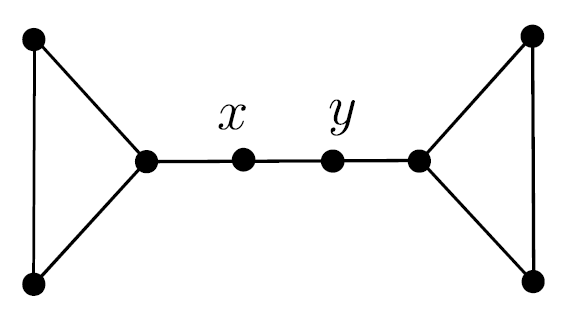
\includegraphics[width=0.3\textwidth]{figs/pblm5.png}
    \caption{Network for problem 5}
    \label{fig:pblm5}
\end{figure}

% \subsection*{Preliminaries:}
% Include Theorems related to requirements to switched system stability... 
% 
% Ideally should put in these theorems....
% 


\subsection*{Solution:}
Within this switched system shown in \figurename \ref{fig:pblm5}, the exclusion of nodes $x$ and $y$ during any singe time-step causes the system to be disconnected into 2 connected subgraphs. 
It is known that consensus will occur within a time-varying (switched) system if the union of multiple time steps cause the network to be connected; 
however, this does not immediately prove this network will converge since the problem statement does not state either x or y will be included.

{\color{red}
    Actually... since at any time-point the node $x$ or $y$ will be missing, the edge $(x,y)$ will never exist.
    This means that even in the case that the two sides wil \textbf{never} be connected.
}


% Problem 6 -------------------------------------------------
\newpage
\section{}
\subsection*{Problem:}
Assume we are running the (directed) consensus protocol over the three static graphs below.
In which of these cases does the protocol drive the state to $\text{span}\vb{1}$?
When does it drive the state to \[
    \frac{1}{N} \vb{1} \vb{1}^T x(0)
\] i.e. to the initial centroid?
(Explain the reasons for your answers - don't just state the answer.)

\subsection*{Preliminaries:}
\begin{definition} 
    Let directed network (di-graph) $G(V,E)$ with $V = \qty{v_1,\dots,v_n}$ and $E \subseteq V \cross V$.
    \begin{enumerate}
        \item A directed path ($P : v_i \to v_j$) is a sequence of directed edges constructing a path from $v_i$ to $v_j$.
        \item 
    \end{enumerate}
\end{definition}

\begin{definition}
    \textbf{Connectivity of Directed Graphs:} 
    Let directed network (di-graph) $G(V,E)$ with $V = \qty{v_1,\dots,v_n}$ and $E \subseteq V \cross V$.
    \begin{enumerate}
        \item Di-graph $G(V,E)$ is \emph{\underline{strongly connected}} there exists a directed path from any node to every other node.
        \item Di-graph $G(V,E)$ is \emph{\underline{weakly connected}} the corresponding undirected graph is connected.
        \item Di-graph $G(V,E)$ is contains a \underline{\emph{rooted out-branching}} if \begin{enumerate}
            \item $G(V,E)$ does not contain a directed cycle
            \item $\exists_{v_r \in V}$ such that $\forall_{v_i \neq v_r \in V}$ there is a directed path from $v_r$ to $v_i$.
        \end{enumerate}
        \item  Di-graph $G(V,E)$ is considered \underline{\emph{balanced}} if $\deg^{in}(v_k) = \deg^{out}(v_k) \forall_{v_k \in V}$.
    \end{enumerate}
\end{definition}

\begin{theorem}
    \textbf{Consensus Requirements:}
    Let directed network (di-graph) $G(V,E)$ with $V = \qty{v_1,\dots,v_n}$ and $E \subseteq V \cross V$
    \begin{enumerate}
        \item 
        \item Di-graph $G(V,E)$ drives to $x$ to $\frac{1}{N} \vb{1} \vb{1}' x(0)$ iff $L$ is balanced and contains a rooted out-branching.
    \end{enumerate}
\end{theorem}

\subsection*{Solution:}
\subsection{$G_1$}
\begin{figure}[h]
    \centering
    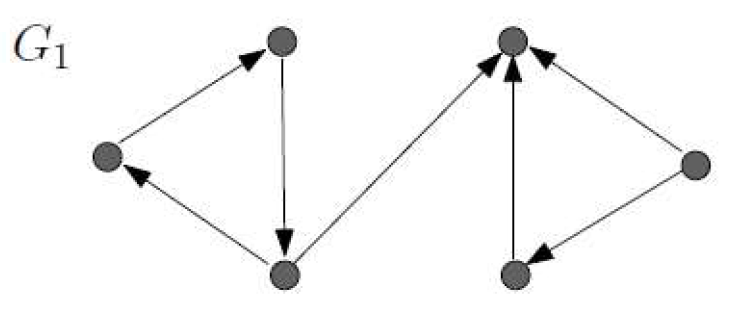
\includegraphics[width=0.5\textwidth]{figs/pblm6a.png}
    % \caption{$G_1$ for Problem 6}
\end{figure}

\[
    D = \mqty[
        -1 & 0  & 1  & 0  & 0  & 0  & 0  \\
        1  & -1 & 0  & 0  & 0  & 0  & 0  \\
        0  & 1  & -1 & -1 & 0  & 0  & 0  \\
        0  & 0  & 0  & 1  & 1  & -1 & 0  \\
        0  & 0  & 0  & 0  & 0  & 1  & 1  \\
        0  & 0  & 0  & 0  & -1 & 0  & -1
    ]
\]\[
    A = \mqty[
        0 & 1 & 0 & 0 & 0 \\
        0 & 0 & 1 & 0 & 0 \\
        1 & 0 & 0 & 1 & 0 \\
        0 & 0 & 0 & 0 & 0 \\
        0 & 0 & 0 & 1 & 0 \\
        0 & 0 & 0 & 1 & 1
    ]
\]\[
    \Delta^{\text{in}} = \mqty[
        1 & 0 & 0 & 0 & 0 & 0 \\
        0 & 1 & 0 & 0 & 0 & 0 \\
        0 & 0 & 2 & 0 & 0 & 0 \\
        0 & 0 & 0 & 0 & 0 & 0 \\
        0 & 0 & 0 & 0 & 1 & 0 \\
        0 & 0 & 0 & 0 & 0 & 2
    ]
\]\[
    L = \mqty[
        1  & -1 & 0  & 0  & 0  & 0 \\
        0  & 1  & -1 & 0  & 0  & 0 `\\
        -1 & 0  & 2  & -1 & 0  & 0 \\
        0  & 0  & 0  & 0  & 0  & 0 \\
        0  & 0  & 0  & -1 & 1  & 0 \\
        0  & 0  & 0  & -1 & -1 & 2
    ]
\] \[
    \text{rank}(L) = 5 = N-1 \implies \text{null}(L) = \text{span}(\vb{1})
\] This means $G_1$ \sout{has rooted out-branching and consensus will occur to $\text{span}(\vb{1})$.
However, $L$ is not balenced as $\deg^{in}(v_k) \neq \deg^{out}(v_k) \forall_{v_k \in V}$, {\color{red} and so it will not converge to the centroid.}
}

{\color{red}
    Looking at the graph it is \textbf{OBVIOUS} that it has a directed cycle (right there on the left) and therefore it does not have rooted out-branching.
    This means that it will not actually converge.
}


\newpage
\subsection{$G_2$}
\begin{figure}[h]
    \centering
    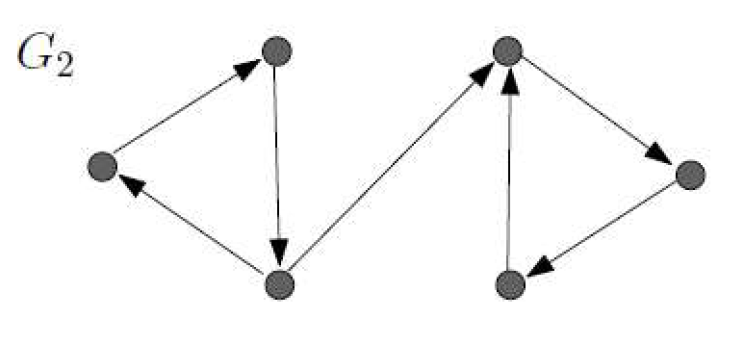
\includegraphics[width=0.5\textwidth]{figs/pblm6b.png}
\end{figure}

\[
    D = \mqty[
        -1 & 0  & 1  & 0  & 0  & 0  & 0  \\
        1  & -1 & 0  & 0  & 0  & 0  & 0  \\
        0  & 1  & -1 & -1 & 0  & 0  & 0  \\
        0  & 0  & 0  & 1  & 1  & -1 & 0  \\
        0  & 0  & 0  & 0  & 0  & 1  & 1  \\
        0  & 0  & 0  & 0  & -1 & 0  & -1
    ]
\]\[
    A = \mqty[
        0 & 1 & 0 & 0 & 0 & 0 \\
        0 & 0 & 1 & 0 & 0 & 0 \\
        1 & 0 & 0 & 1 & 0 & 0 \\
        0 & 0 & 0 & 0 & 1 & 0 \\
        0 & 0 & 0 & 0 & 0 & 0 \\
        0 & 0 & 0 & 1 & 1 & 0
    ]
\]\[
    \Delta^{\text{in}} = \mqty[
        1 & 0 & 0 & 0 & 0 & 0 \\
        0 & 1 & 0 & 0 & 0 & 0 \\
        0 & 0 & 2 & 0 & 0 & 0 \\
        0 & 0 & 0 & 1 & 0 & 0 \\
        0 & 0 & 0 & 0 & 0 & 0 \\
        0 & 0 & 0 & 0 & 0 & 2
    ]
\]\[
    L = \mqty[
        1  & -1 & 0  & 0  & 0  & 0 \\
        0  & 1  & -1 & 0  & 0  & 0 \\
        -1 & 0  & 2  & -1 & 0  & 0 \\
        0  & 0  & 0  & 1  & -1 & 0 \\
        0  & 0  & 0  & 0  & 0  & 0 \\
        0  & 0  & 0  & -1 & -1 & 2
    ]
\] \[
    \text{rank}(L) = 5 = N-1 \implies \text{null}(L) = \text{span}(\vb{1})
\] This means $G_2$ has rooted out-branching and consensus will occur to $\text{span}(\vb{1})$.
However, $L$ is not balenced as $\deg^{in}(v_k) \neq \deg^{out}(v_k) \forall_{v_k \in V}$ {\color{red} and so it will not converge to the centroid.}

\newpage
\subsection{$G_3$}
\begin{figure}[h]
    \centering
    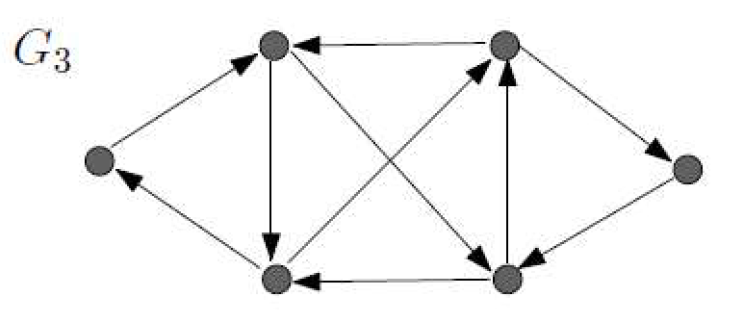
\includegraphics[width=0.5\textwidth]{figs/pblm6c.png}
\end{figure}

\[
    D = \mqty[
        -1 & 0  & 1  & 0  & 0  & 0  & 0  & 0  & 0  & 0  \\
        1  & -1 & 0  & 0  & 0  & 0  & 0  & 1  & -1 & 0  \\
        0  & 1  & -1 & -1 & 0  & 0  & 0  & 0  & 0  & 1  \\
        0  & 0  & 0  & 1  & 1  & -1 & 0  & -1 & 0  & 0  \\
        0  & 0  & 0  & 0  & 0  & 1  & -1 & 0  & 0  & 0  \\
        0  & 0  & 0  & 0  & -1 & 0  & 1  & 0  & 1  & -1
    ]
\]\[
    A = \mqty[
        0 & 1 & 0 & 0 & 0 & 0 \\
        0 & 0 & 1 & 0 & 0 & 1 \\
        1 & 0 & 0 & 1 & 0 & 0 \\
        0 & 1 & 0 & 0 & 1 & 0 \\
        0 & 0 & 0 & 0 & 0 & 1 \\
        0 & 0 & 1 & 1 & 0 & 0
    ]
\]\[
    \Delta^{\text{in}} = \mqty[
        1 & 0 & 0 & 0 & 0 & 0 \\
        0 & 2 & 0 & 0 & 0 & 0 \\
        0 & 0 & 2 & 0 & 0 & 0 \\
        0 & 0 & 0 & 2 & 0 & 0 \\
        0 & 0 & 0 & 0 & 1 & 0 \\
        0 & 0 & 0 & 0 & 0 & 2
    ]
\]\[
    L = \mqty[
        1  & -1 & 0  & 0  & 0  & 0  \\
        0  & 2  & -1 & 0  & 0  & -1 \\
        -1 & 0  & 2  & -1 & 0  & 0  \\
        0  & -1 & 0  & 2  & -1 & 0  \\
        0  & 0  & 0  & 0  & 1  & -1 \\
        0  & 0  & -1 & -1 & 0  & 2
    ]
\] \[
    \text{rank}(L) = 5 = N-1 \implies \text{null}(L) = \text{span}(\vb{1})
\] This means $G_3$ has rooted out-branching and consensus will occur to $\text{span}(\vb{1})$.
Additionally, $L$ is balanced as $\deg^{in}(v_k) = \deg^{out}(v_k) \forall_{v_k \in V}$
{\color{red} and so it will therefore converge to the centroid of the initial positions.}




% Problem 7 -------------------------------------------------
\newpage
\section{}
\subsection*{Problem:}
Show that a graph that is weakly connected and balanced is also strongly connected.
(
    I do not expect a formal proof.
    % \footnote{
    %     Nah...
    % }
    Just discuss your main argument.
    % \footnote{
    %     This sounds more difficult then actually proving it.
    % }
)

% \subsection*{Preliminaries:}
% 
% 
% 
% should probably do the theorems in this....
% 
% 


\subsection*{Solution:}
\begin{theorem}
    Let graph $G(V,E)$ with $V = \qty{v_1,\dots,v_n}$ and $E \subseteq V \cross V$.

    If $G(V,E)$ is weakly connected and balanced, then $G(V,E)$ is strongly connected.
    (i.e)\[
        G(V,E) \text{Weakly Connected} 
            \land G(V,E) \text{Balanced}
            \implies G(V,E) \text{Strongly Connected}
    \]
    \begin{proof}
        Not a formal proof...
        Essentially the related undirected network being fully connected, as implied by weakly connected, is then connected to the fact that the network is balanced implying in and out degrees are the same with can be used to prove directed paths exist in addition to just undirected connectivity.
    \end{proof}
\end{theorem}



\subsection*{\color{red} Actual Solution:}
Steps:
\begin{enumerate}
    \item Show that if a graph is balanced then $\forall_{v \in V} \exists$ a directed cycle containing $v$.
    \item Demonstrate that being weakly connected implies the cycles overlap.
    \item These cycles then form a path from every node to every other node.
\end{enumerate}



\newpage
\appendix
\section{MATLAB Code:}\label{apx:matlab}
All code I write in this course can be found on my GitHub repository:\\
\href{https://github.com/jonaswagner2826/MECH6V29_MultiagentRoboticSystems}{https://github.com/jonaswagner2826/MECH6V29\_MultiagentRoboticSystems}

% \bibliographystyle{ieeetran}
% % \bibliography{refs.bib}
% \cite{*}

% 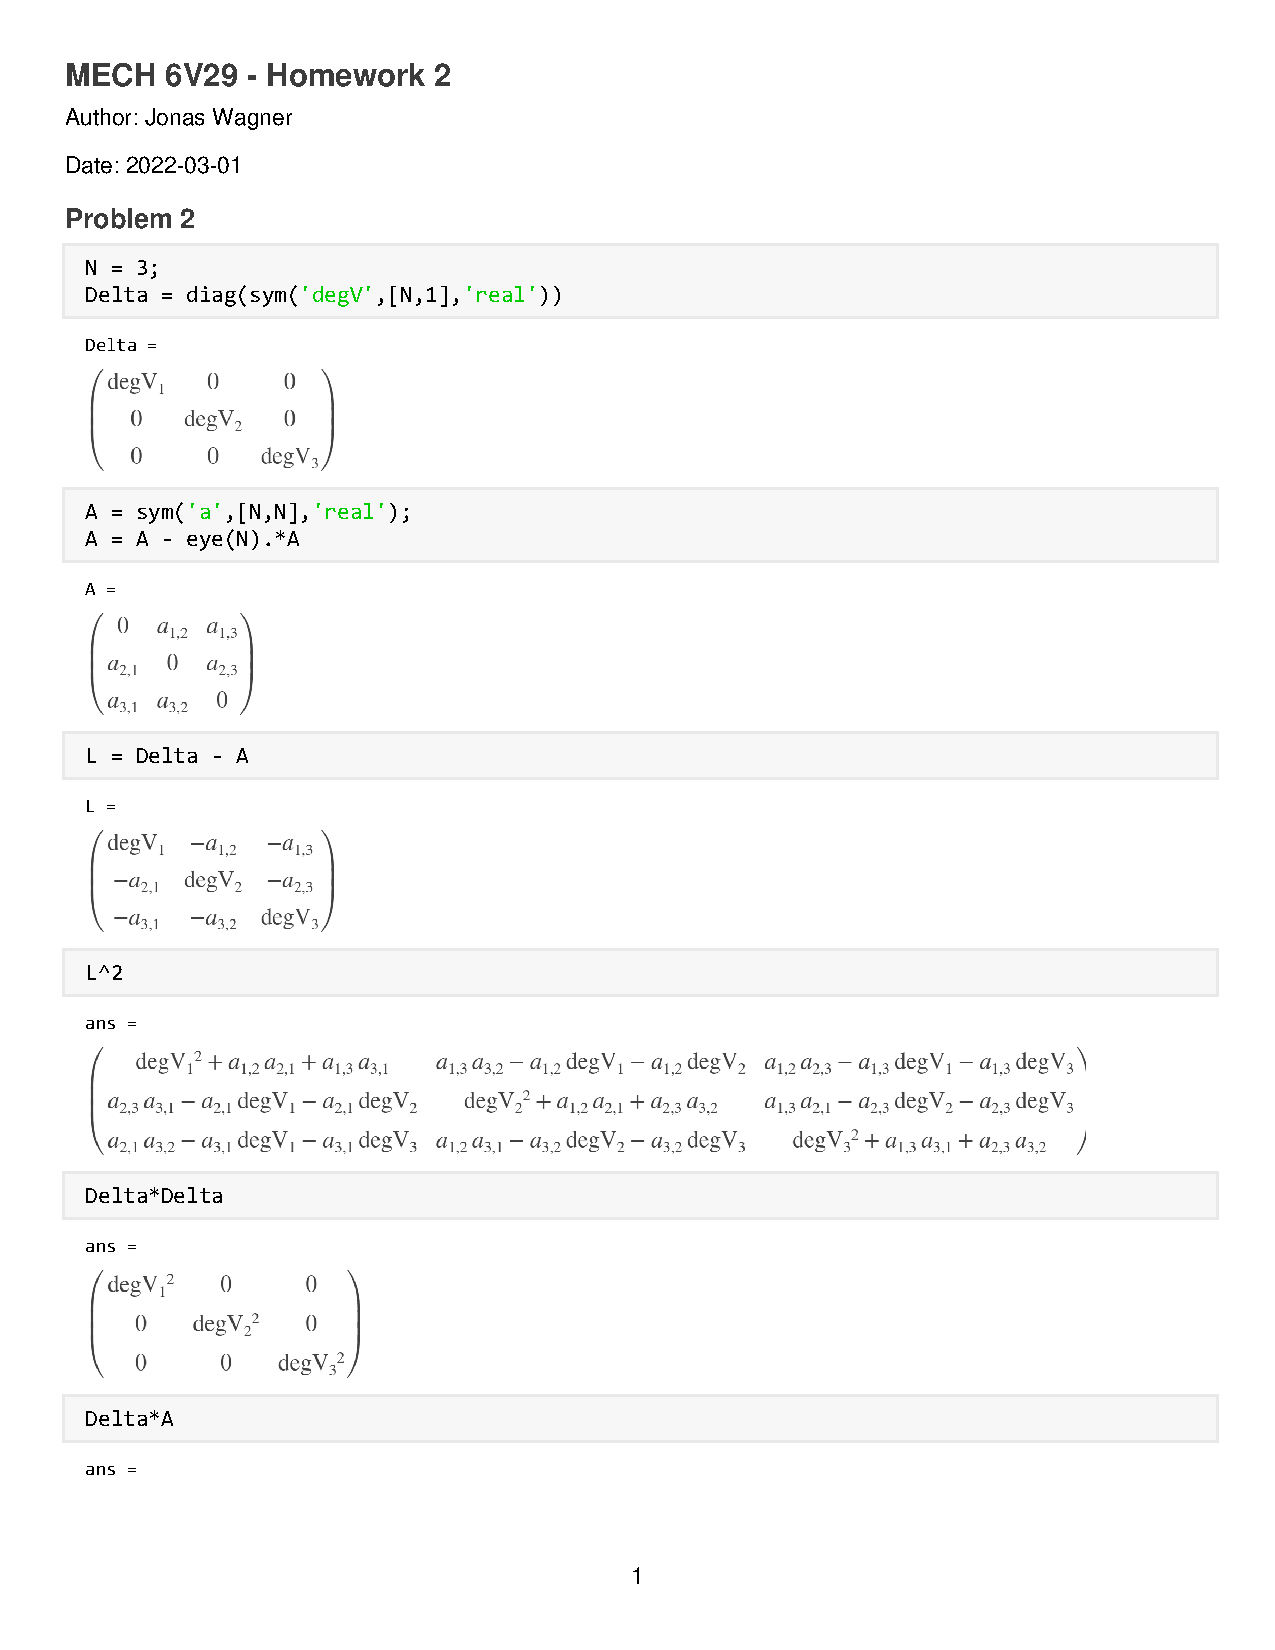
\includepdf[pages=-]{MECH6V29_HW02.pdf}
% 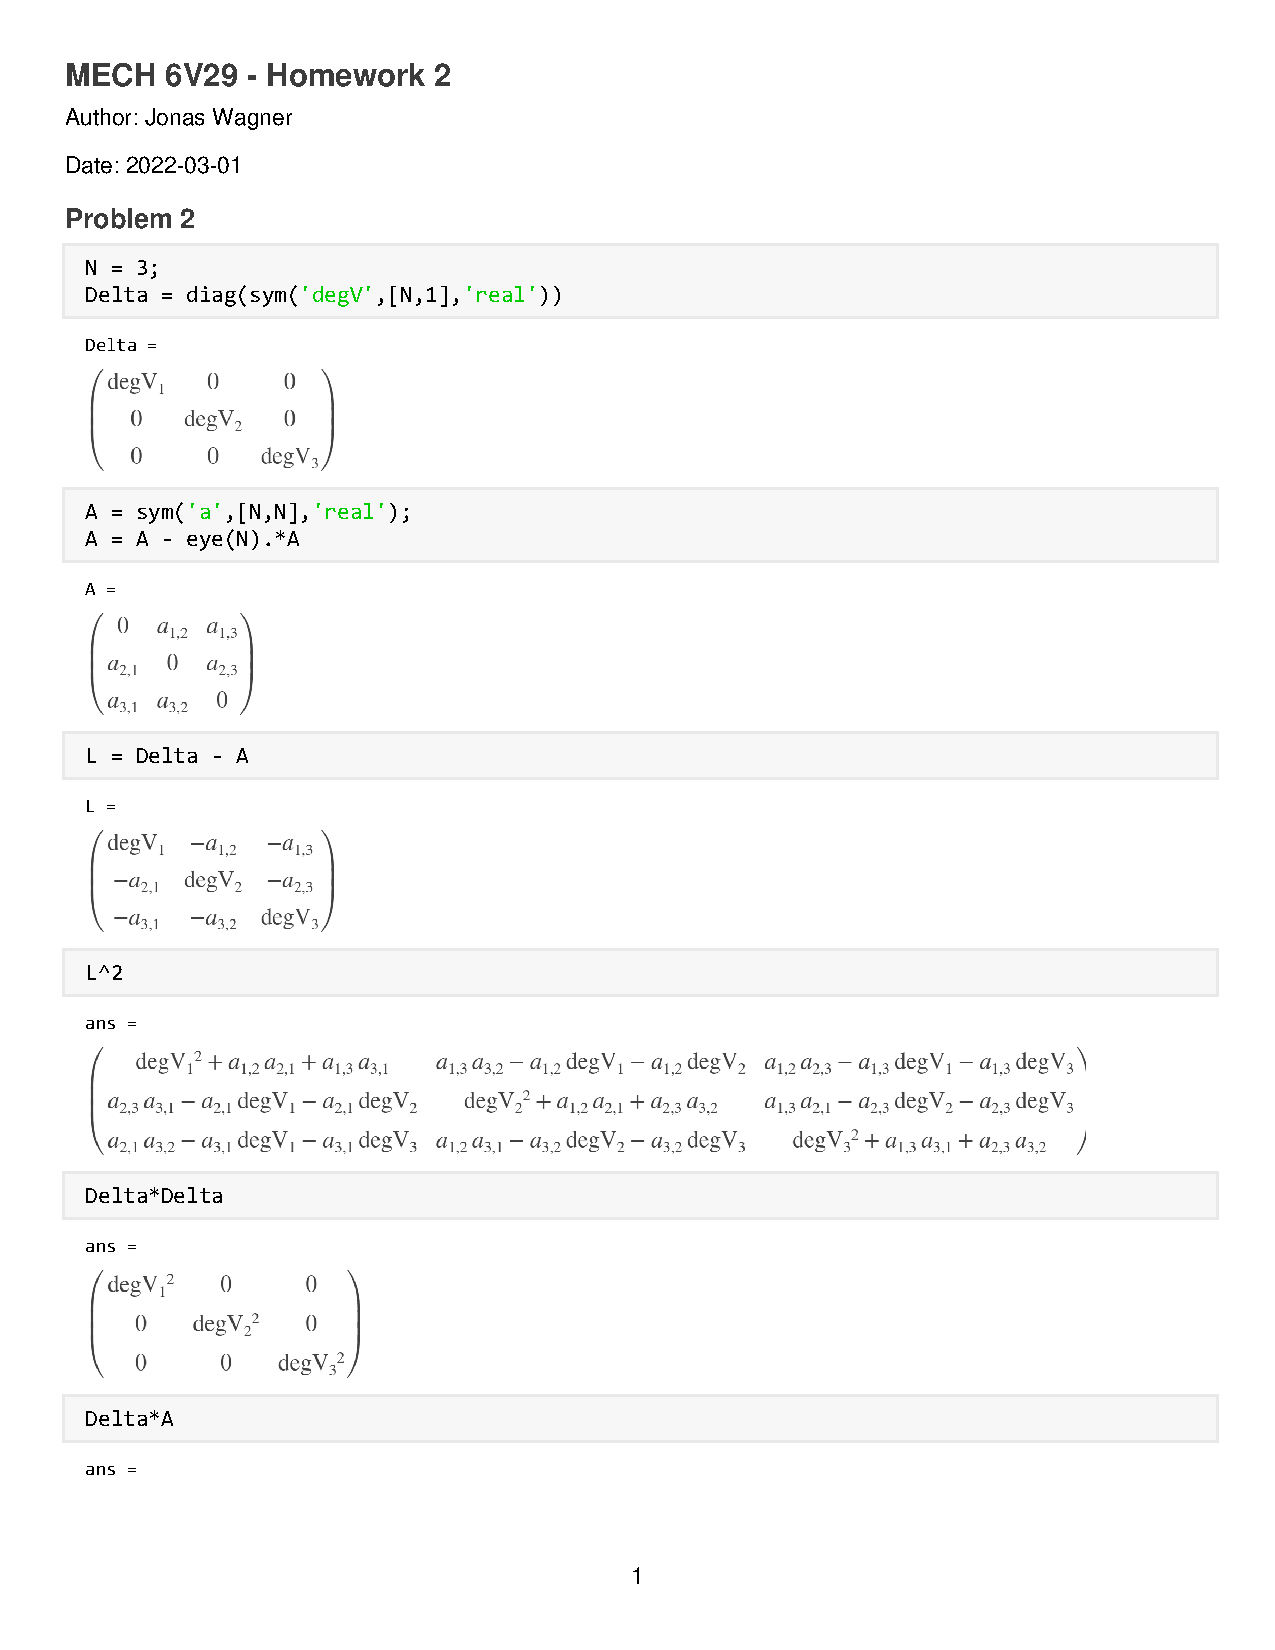
\includepdf[pages=-, nup = 2x2]{MECH6V29_HW02.pdf}


\end{document}
